\documentclass{article}
\usepackage{graphicx}
\usepackage{amsmath}
\usepackage{float}
\usepackage{qcircuit}
\usepackage{hyperref}
\usepackage{graphicx}
\usepackage{rotating}
\usepackage{pdflscape}
\usepackage{multirow,tabularx}
\usepackage{authblk}
\usepackage{amsthm}
\usepackage{caption}
\usepackage{subcaption}
\usepackage{tabularx}
\usepackage{cite}
\usepackage{color}

\usepackage[no-files]{xsim}
\usepackage{needspace}
\usepackage{tasks}

\DeclareExerciseEnvironmentTemplate{custom}{%
  \par\vspace{\baselineskip}
  \Needspace*{2\baselineskip}
  \noindent\sffamily
  \textbf{\XSIMmixedcase{\GetExerciseName}~\GetExerciseProperty{counter}}%
  \GetExercisePropertyT{subtitle}{\hspace{3em}{\small#1}}\par
  \normalfont
}{}

\DeclareExerciseEnvironmentTemplate{flushright}{%
  \begin{flushright}
  \begin{minipage}{.4\linewidth}
    \textsf{Solutions:}\par\normalfont
}{%
  \end{minipage}%
  \end{flushright}%
}

\xsimsetup{
  exercise/within = section ,
  exercise/template = custom ,
  solution/template = flushright
}

\renewcommand*\theexercise{\arabic{exercise}}

\newcommand\QA[2]{\IfInsideSolutionTF{#2}{#1}}

\begin{document}


% \setcounter{section}{1}
% \setcounter{exercise}{1}

\begin{exercise}[subtitle = IBM Q2 and the Hard Mapping Problem]
IBM recently has provided the world with one of the first quantum computers. Even though it is not one of the powerful quantum computers available in the market, but it has proven the world it is possible to construct such devices. Unfortunately, this quantum computer comes with very restrictive interactions. Take for example the \textit{IBM Q2} illustrated in Figure \ref{fig:ibmq2}, it has restrictions on the interactions between qubits. For example, $Q0$ can be the control qubit for $Q1$ and $Q2$; $Q2$ can be the target qubit for both $Q0$ and $Q1$. $Q1$ can be both a target qubit and a control qubit; \textit{i.e.}, the arrows depicted in Figure \ref{fig:ibmq2} illustrate the restrictions of interactions between qubits. 


Given the circuit in Figure \ref{fig:exercise1}, map it on IBM Q2 using as minimum quantum gates as possible.You may use the variations of SWAP gates in Figure \ref{fig:swap-gates} as a workaround to connect qubits.

\begin{figure}[H]
    \centering
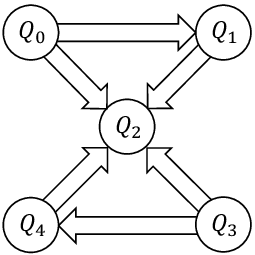
\includegraphics[width=2.5cm, height=2.5cm]{assets/images/The-architecture-of-IBM-Q-Experiences-5-qubit-quantum-computer-IBMQX2-cited-from-20.png}

    \caption{IBM Q2 quantum computer. \label{fig:ibmq2}}
\end{figure}



\begin{figure}[H]
        \begin{align*}
            \Qcircuit @C=1.0em @R=1em @!R{
               \lstick{x_0} &\qw&\qw&\targ&\qw&\qw&\qw\\ 
               \lstick{x_1}  &\qw&\qw&\ctrl{ -1 }&\ctrl{ 3 }&\qw&\qw\\ 
               \lstick{x_2}  &\qw&\ctrl{ 1 }&\qw&\qw&\ctrl{ 1 }&\qw\\ 
               \lstick{x_3}  &\qw&\targ&\qw&\qw&\targ&\qw\\ 
               \lstick{x_4}  &\qw&\qw&\qw&\targ&\qw&\qw\\ 
            }
        \end{align*}
        \caption{Map this circuit on \textit{IBM Q2},  where $\oplus$ is the XOR-operation. \label{fig:exercise1}}
\end{figure}


\begin{figure}[H]
\centering

% \hfill
\begin{subfigure}[b]{0.4\textwidth}
        \begin{align*}
        \Qcircuit @C=1.0em @R=1em @!R{
       \lstick{A} &\qw&\ctrl{1}&\gate{H}&\ctrl{ 1 }&\gate{H}&\ctrl{1}&\qw & \rstick{B}\\ 
       \lstick{B} &\qw&\targ&\gate{H}&\targ&\gate{H}&\targ&\qw & \rstick{A}\\ 
        }
\end{align*}

\end{subfigure}
\hfill
\begin{subfigure}[b]{0.4\textwidth}
        \begin{align*}
        \Qcircuit @C=1.0em @R=1em @!R{
            \lstick{A} &\qw&\ctrl{ 1 }&\targ&\ctrl{ 1 }&\qw &\rstick{B}\\ 
            \lstick{B} &\qw&\targ&\ctrl{ -1 }&\targ&\qw & \rstick{A}\\ 
        }
        \end{align*}
\end{subfigure}
\caption{Variations of SWAP gates, where $H$ is Hadamard gate. \label{fig:swap-gates}}
\end{figure}

\end{exercise}

\begin{exercise}[subtitle = The John Doe Circuit]
While searching online, to satisfy your sense of curiosity about quantum, you stumped upon the circuit in Figure \ref{fig:john-doe}. You're interested to know what computations it performs on the input. Trace this circuit to find the output. You may use the gates provided in Figure \ref{fig:qgates}.

\begin{figure}[H]
    \begin{align*}
        \Qcircuit @C=1.0em @R=1em @!R{
            \lstick{A}   &\qw&\targ&\qw&\qw&\qw\\ 
            \lstick{B}  &\qw&\ctrl{ -1 }&\targ&\qw&\qw\\ 
            \lstick{C}  &\qw&\ctrl{ -2 }&\ctrl{ -1 }&\targ&\qw\\ 
        }
        \end{align*}
        \caption{The John Doe circuit. \label{fig:john-doe}}
\end{figure}
\end{exercise}

\begin{exercise}[subtitle = The Jane Doe Black-Box Circuit]
A black-box circuit is a circuit hidden in an unbreakable box which means you cannot open the black-box and see how qubits interact with each other and which gates are used as well,\textit{ i.e.}, everything is hidden from sight. This black-box promises to output certain Boolean functions on every output qubit, given an input. Given the black-box in Figure \ref{fig:jane-doe}, try to reverse-engineer the output to get the circuit that performs this Boolean operations with as minimum gates as possible. You may use the gates provided in Figure \ref{fig:qgates}.


\begin{figure}[H]
    \begin{align*}
        \Qcircuit @C=1.0em @R=1em @!R{
            \lstick{A}&\qw&\multigate{3}{Jane Doe}&\qw &  \rstick{A}\\ 
            \lstick{B} &\qw&\ghost{Jane Doe}&\qw & \rstick{A\oplus B}\\ 
            \lstick{0} &\qw&\ghost{Jane Doe}&\qw & \rstick{A\oplus B \oplus C}\\ 
            \lstick{C} &\qw&\ghost{Jane Doe}&\qw & \rstick{AB\oplus  C\oplus 1 }\\ 
        }
        \end{align*}
        \caption{The Jane Doe Black-box. \label{fig:jane-doe}}
\end{figure}

\begin{figure}[H]
    % \centering
    \begin{subfigure}[b]{0.3\textwidth}
        
        \begin{align*}
            \Qcircuit @C=1.0em @R=1em @!R{
           \lstick{A} &\qw&\ctrl{ 2 }&\qw & \rstick{A}\\ 
           \lstick{B} &\qw&\ctrl{ 1 }&\qw & \rstick{B}\\ 
           \lstick{C} &\qw&\targ&\qw & \rstick{AB\oplus C}\\ 
        }
        \end{align*}
        \caption{The Toffoli gate. }
        \label{fig:toffoli}
    \end{subfigure}
\hfill
    \begin{subfigure}[b]{0.3\textwidth}
        \begin{align*}
            \Qcircuit @C=1.0em @R=1em @!R{
                \lstick{A} &\qw&\ctrl{ 1 }&\qw &  \rstick{A}\\ 
                \lstick{B} &\qw&\targ&\qw & \rstick{A\oplus B}\\ 
            }
            \end{align*}
            \caption{The \textit{CNOT} gate.}
            \label{fig:cnot}
\end{subfigure}
\hfill
    \begin{subfigure}[b]{0.3\textwidth}
        \begin{align*}
            \Qcircuit @C=1.0em @R=1em @!R{
                \lstick{A} &\qw&\targ&\qw &  \rstick{A\oplus 1}\\ 
            }
            \end{align*}
            \caption{The \textit{CNOT} gate.}
            \label{fig:not}
\end{subfigure}

\caption{Some $1$-bit, $2$-bit, and $3$-bit quantum gates and their outputs. \label{fig:qgates}}

\end{figure}

\end{exercise}

\begin{exercise}[subtitle = Mathematics of Quantum States]

    \begin{tasks}

   

\task For each of the following qubits, if a measurement is made, what is the probability that we find the qubit in state $\vert 0\rangle$? What is the probability that we find the qubit in the state $\vert 1\rangle$ ?


\begin{enumerate}
    \item $\vert \psi\rangle = \frac{1}{\sqrt{3}}\vert 0\rangle +  \sqrt{\frac{2}{3}}\vert 1\rangle$.
    \item $\vert  \phi \rangle = \frac{i}{2} \vert 0\rangle + \frac{\sqrt{3}}{2}\vert 1\rangle $.
    \item $\vert \chi \rangle = \frac{(1+i)}{\sqrt{3}} \vert 0\rangle - \frac{i}{\sqrt{3}} \vert 1\rangle$
\end{enumerate}


\task If $\vert \psi \rangle=\frac{1}{2} (\vert 0\rangle \vert 0\rangle - \vert 0\rangle\vert 1\rangle +\vert 1\rangle \vert 0\rangle - \vert 1\rangle  \vert 1\rangle)$, could it be written as a product state?


\task Calculate the tensor product of


\begin{align*}
    \vert a\rangle \frac{1}{\sqrt{2}}\begin{bmatrix}
        1 \\ -1
    \end{bmatrix}
\end{align*}
and

\begin{align*}
    \vert b\rangle \frac{1}{\sqrt{3}}\begin{bmatrix}
        \sqrt{2} \\ 1
    \end{bmatrix}
\end{align*}


\task Suppose $\varphi\rangle =\vert a\rangle \otimes \vert b\rangle $ and $A\vert a\rangle = a\vert a\rangle$, $B\vert b\rangle = b\vert b\rangle$. What is $A\otimes B\vert \varphi\rangle$.


\task Find $X\otimes Z\vert \psi\rangle$, where $\vert \psi\rangle = \frac{\vert 0\rangle \vert 0\rangle - \vert 1\rangle \vert 1\rangle}{\sqrt{2}}$.



\task Suppose that

\begin{align*}
    \vert \psi \rangle = \frac{\vert 00\rangle - \vert 11\rangle}{\sqrt{2}},
\end{align*}
describe the action of $X\otimes I$ on the given state.


\task Show that $(A\otimes B)^\dagger = A^\dagger \otimes B^\dagger$.


\end{tasks}
\end{exercise}

\end{document}